\documentclass[a4paper]{article} 
\addtolength{\hoffset}{-2.25cm}
\addtolength{\textwidth}{4.5cm}
\addtolength{\voffset}{-3.25cm}
\addtolength{\textheight}{5cm}
\setlength{\parskip}{0pt}
\setlength{\parindent}{0in}

%----------------------------------------------------------------------------------------
%	PACKAGES AND OTHER DOCUMENT CONFIGURATIONS
%----------------------------------------------------------------------------------------

\usepackage{blindtext} % Package to generate dummy text
\usepackage{charter} % Use the Charter font
\usepackage[utf8]{inputenc} % Use UTF-8 encoding
\usepackage{microtype} % Slightly tweak font spacing for aesthetics
\usepackage[english, ngerman]{babel} % Language hyphenation and typographical rules
\usepackage{amsthm, amsmath, amssymb} % Mathematical typesetting
\usepackage{float} % Improved interface for floating objects
\usepackage[final, colorlinks = true, 
            linkcolor = black, 
            citecolor = black]{hyperref} % For hyperlinks in the PDF
\usepackage{graphicx, multicol} % Enhanced support for graphics
\usepackage{xcolor} % Driver-independent color extensions
\usepackage{marvosym, wasysym} % More symbols
\usepackage{rotating} % Rotation tools
\usepackage{censor} % Facilities for controlling restricted text
\usepackage{listings, style/lstlisting} % Environment for non-formatted code, !uses style file!
\usepackage{pseudocode} % Environment for specifying algorithms in a natural way
\usepackage{style/avm} % Environment for f-structures, !uses style file!
\usepackage{booktabs} % Enhances quality of tables
\usepackage{tikz-qtree} % Easy tree drawing tool
\tikzset{every tree node/.style={align=center,anchor=north},
         level distance=2cm} % Configuration for q-trees
\usepackage{style/btree} % Configuration for b-trees and b+-trees, !uses style file!
\usepackage[backend=biber,style=numeric,
            sorting=nyt]{biblatex} % Complete reimplementation of bibliographic facilities
\addbibresource{ecl.bib}
\usepackage{csquotes} % Context sensitive quotation facilities
\usepackage[yyyymmdd]{datetime} % Uses YEAR-MONTH-DAY format for dates
\renewcommand{\dateseparator}{-} % Sets dateseparator to '-'
\usepackage{fancyhdr} % Headers and footers
\pagestyle{fancy} % All pages have headers and footers
\fancyhead{}\renewcommand{\headrulewidth}{0pt} % Blank out the default header
\fancyfoot[L]{} % Custom footer text
\fancyfoot[C]{} % Custom footer text
\fancyfoot[R]{\thepage} % Custom footer text
\newcommand{\note}[1]{\marginpar{\scriptsize \textcolor{red}{#1}}} % Enables comments in red on margin

%----------------------------------------------------------------------------------------

\begin{document}

%-------------------------------
%	TITLE SECTION
%-------------------------------

\fancyhead[C]{}
\hrule \medskip % Upper rule
\begin{minipage}{0.295\textwidth} 
\raggedright
\footnotesize
\textbf{Pedro Luis Lobato Barros} \hfill\\    
202012490\hfill\\
p.lobato

\textbf{Jaime Andres Torres Bermejo} \hfill\\   
202014866\hfill\\
j.torres16

\textbf{Sofia Torres Ramírez} \hfill\\   
202014872\hfill\\
s.torres21

\end{minipage}
\begin{minipage}{0.4\textwidth} 
\centering 
\large 
Caso 1\\ 
\normalsize 
Infraestructura Computacional - Universidad de los Andes\\ 
\end{minipage}
\begin{minipage}{0.295\textwidth} 
\raggedleft
\today\hfill\\
\end{minipage}
\medskip\hrule 
\bigskip

%-------------------------------
%	CONTENTS
%-------------------------------

\section{Estructura del Proyecto}
    
    \subsection{UML}
    Por medio de este diagrama UML se puede entender a grandes rasgos el funcionamiento del programa. Iniciando por la clase “Process” Podemos ver que esta clase extiende de “Runnable”.  Siguiendo con esta Idea, las clases “Orange”, “Blue” y “Red” al representar los diferentes procesos que puede tener el programa implementarán a la clase “Process”. Tal como lo evidencia el diagrama, las clases “Orange” y “Blue” tienen el mismo objetivo final, procesar productos. Sin embargo, su funcionamiento interno es diferente y este se especificará más adelante. Los atributos de estas clases son:  
    
    \begin{enumerate}
        \item “msgLimit”: El número de productos o mensajes que se deben crear por cada tipo de proceso y que por ende se deben imprimir al finalizar el programa. Este atributo es estático por lo tanto está subrayado y solo se puede leer, no modificar.  
        \item “Id”: El identificador de cada proceso creado. 
        \item “stage”: El identificador de la etapa en la cual se encuentra el proceso creado. 
        \item “timeMillis”: El tiempo que debe dormir el proceso para simular la modificación del mensaje/producto. 
    \end{enumerate}
    Estos 4 atributos son iguales tanto para el proceso azul como para el naranja. El proceso rojo no tiene los atributos “stage”, “id” y “timeMillis” debido a que solo se crea un proceso rojo, el cual no necesitaría un id para diferenciarse. Se sabe que estará en la parte final del proceso por ende no es necesario especificar su etapa y al no modificar el mensaje no necesita un tiempo durante el cual simular esta modificación. Sin embargo, tiene un atributo adicional llamado “process” el cual tiene la información de cuantos procesos están activos. 

    Con respecto a la clase “Buffer” podemos ver que tiene los siguientes atributos: 
    \begin{enumerate}
        \item “MAX_SIZE”: La capacidad del buffer. 

        \item “queueOrange”: Una cola que almacena los productos/mensajes que fueron creados y modificados por procesos naranjas. 
        
        \item “queueBlue”: Una cola que almacena los productos/mensajes que fueron creados y modificados por procesos azules. 
        
        \item “occupied”: La cantidad de productos/mensajes que hay en el buffer. 
    \end{enumerate}
     

    Tanto el proceso naranja (Orange) como el azul (Blue) tienen dos relaciones con el Buffer. Una de estas relaciones representa el buffer de entrada, es decir, el Buffer del cual se sacan los mensajes para modificarlos. La cardinalidad de estas relaciones es de 0..1 debido a que si el proceso corresponde a la etapa 0, no existiría buffer de entrada ya que en esta etapa se crean los procesos. De lo contrario, es decir, si un proceso no pertenece al la etapa 0, siempre existirá un “Buffer in” del cual sacar los mensajes. Por otro lado, para todo proceso Azul o Naranja siempre existirá un “Buffer out” o Buffer de salida, en el cual se colocarán los mensajes ya modificados o recién creados para que un proceso de la siguiente etapa lo pueda coger y modificar. 

    Sin embargo, el proceso rojo no funciona igual debido a que este proceso solo tendrá interacción con el último Buffer, del cual sacará los mensajes para luego imprimirlos. 



    \subsection{la clase 'Main'}

    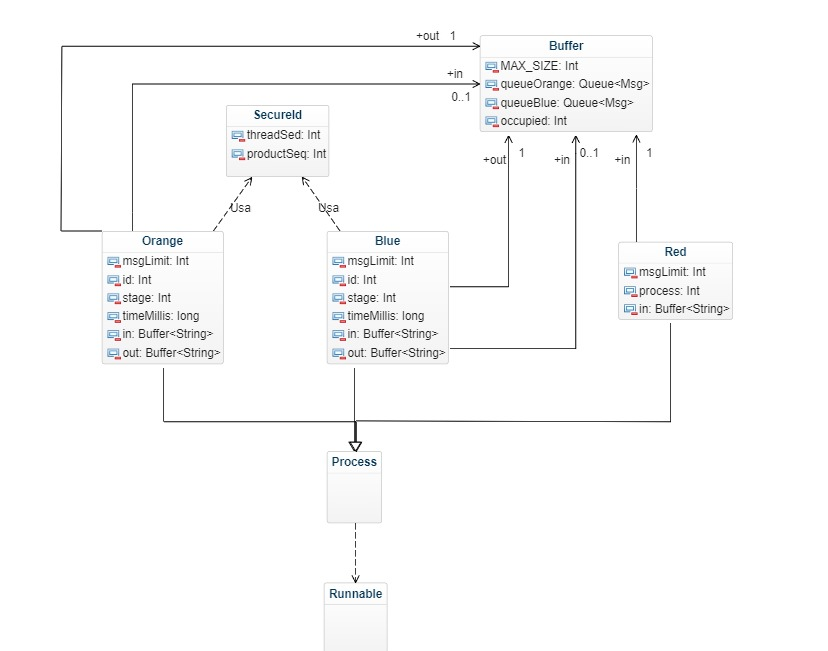
\includegraphics{uml.jpeg}

    La principal función de la clase 'Main', además de correr el programa,
    es unir al resto del programa para su funcionamiento óptimo, en 'Main.java'
    esta definida la estructura que las clases que vamos a manejar para solucionar
    el problema.

    Una de las primeras cosas que van a saltar a la vista es el uso de constantes
    definidas como 'final' dentro de la lógica de java. con esto, pretendemos 
    hacer que las variables acá definidas sean inmutables y no puedan ser cambiadas
    ni por el usuario ni por ninguno de los procesos que el programa corra una vez
    definidas. Las variables que caen dentro de este conjunto inmutable son

    \begin{enumerate}
        \item texttt{MESSAGE NUM:} Define el número de mensajes a enviar.
        \item texttt{PROCESS NUM:} Define el número de procesos del programa.
        \item texttt{BUFFER CAP:} Define el limite del Buffer
        \item texttt{BUFFER NUM:} Define el número de Buffers
        \item texttt{STAGE NUM:} Define el número de etapas por las que pasarán los procesos
    \end{enumerate}

    Estas conses son luego utilizadas para la creación de los objetos
    que serán usados en el programa, y conectará la lógica de esos
    nuevos objetos creados. 

    \subsection{Estructura de los Procesos}
        \subsubsection{Blue}
        \includegraphics{}
        En la parte inicial del código se puede ver la definición de los atributos de la clase “Blue”, su método constructor y un método para darle valor al atributo “msgLimit”. 
        \includegraphics{}
        Luego de esto podemos ver el método run del proceso, en donde, si la etapa del proceso creado es igual a 0, correrá el método “runZero( )”, de lo contrario, correrá el método “runNonZero( )”. Esto se hace debido a que, si el proceso pertenece a la etapa cero, quiere decir que aun no se han creado los productos/mensajes, por ende, toca crearlos. Si la etapa es diferente de 0, ya están creados los mensajes así que el proceso debería obtenerlos del buffer de entrada. 
        \includegraphics{}
        En la primera parte del método “runNonZero()” se crea un lamda expresion y un objeto anónimo llamado context el cual tendrá dos atributos msg y counter en donde “msg” será el mensaje sacado del buffer de entrada y “counter” será el número de mensajes que se han procesado. Teniendo en cuenta esta información, se ejecutará un ciclo mientras todavía no se hayan procesado todos los mensajes azules. Luego de esto se sincroniza la cola de los mensajes azules del buffer de entrada (in) para asegurar que el recurso solo será manejado por este proceso. Mientras la cola de mensajes azules del buffer de entrada esté vacía el proceso esperará sobre esta cola hasta que otro proceso agregue un mensaje azul a esta y el proceso actual lo pueda tomar. Aquí se puede evidenciar la espera pasiva por parte de los procesos azules debido a que el proceso esperará hasta que le notifiquen, no preguntará constantemente si el buffer ya no está vacío. Cuando la cola no esté vacía, el proceso toma un mensaje, notifica esto a la cola y libera el recurso. 

        En esta parte del código se realiza la transformación necesaria del mensaje agregándole esta nueva etapa por la que pasó y luego el proceso se duerme por un tiempo aleatorio simulando dicha transformación. 

        Luego de modificar el mensaje es necesario agregarlo al buffer de salida (out), debido a esto, primero se sincroniza el buffer para garantizar la obtención del recurso y no leer datos inconsistentes. Luego, se ejecuta un ciclo en donde, si la cola de mensajes azules del buffer de salida está lleno, se notifica que se está intentando agregar un nuevo mensaje a la cola y luego espera a que haya espacio en ella para poder agregar el mensaje. Cuando la cola no está llena se agregará el mensaje modificado y el contador de mensajes procesados aumenta en uno. Luego de esto, se notifica a todos los que estén esperando sobre esta cola por si algún proceso de la siguiente etapa estaba esperando por él. No se realiza un “notify( )” debido a que es posible que se notifique a un proceso que ya halla terminado de procesar sus mensajes. 

        Por último se tiene la función “runZero( )” en donde se crea una lamda expresion u objeto anónimo llamado “context” el cual tiene un atributo llamado “counter” que cuenta la cantidad de productos/mensajes creados. Luego de esto se ejecuta un ciclo mientras el número de mensajes creados sea menor al número de mensajes a crear. Mientras esto suceda se sincroniza la cola de mensajes azules del buffer de salida de la etapa 0 (el cual sería el primer buffer) para garantizar la obtención del recurso. Dentro de esta sincronización se consulta si la cola de mensajes azules está llena, de ser así el proceso espera sobre esta cola hasta que ya no esté llena. Cuando esta cola no está llena, se crea el mensaje y se agrega, luego se aumenta el contador de mensajes creados y se notifica a la cola de mensajes azules del buffer de salida que se agregó el mensaje por si algún proceso de la etapa siguiente estaba esperando por él. 
        
        \subsubsection{Orange}
        En la parte inicial del código se puede ver la definición de los atributos de la clase Orange, su método constructor y un método para darle valor al atributo “msgLimit”. 

        Luego de esto podemos ver el método run del proceso en donde, si la etapa del proceso creado es igual a 0, correrá el método “runZero( )”, de lo contrario correrá el método “runNonZero( )”. Esto se hace debido a que, si el proceso pertenece a la etapa cero, quiere decir que aún no se han creado los productos/mensajes, por ende, toca crearlos. Si la etapa es diferente de 0, ya están creados los mensajes así que el proceso tendría que obtenerlos del buffer de entrada. 

        En la primera parte del método “runNonZero se crea un lamda expresion u objeto anónimo llamado “context” el cual tendrá dos atributos “msg” y “counter”, en donde “msg” será el mensaje sacado del buffer de entrada y “counter” será el número de mensajes que se han procesado. Teniendo en cuenta esta información, luego se ejecutará un ciclo mientras todavía no se hallan procesado todos los mensajes azules. Siguiente a esto se llama a la función lamda “in.synchronizedOrange( )” la cual permite que en el primer bloque de instrucciones aún no se halla sincronizado la cola de mensajes naranjas del buffer de entrada pero en el segundo sí exista esta sincronización. En el primer bloque se evalúa si la cola de mensajes naranjas está vacía. Si esto es cierto, se ejecuta la instrucción “Thread.yield( )” la cual generará que el proceso ceda el procesador y lo vuelva a solicitar inmediatamente para volver a consultar lo mismo hasta que ya no esté vacía. Es aquí en donde se puede evidenciar el comportamiento de espera semiactiva por parte del proceso naranja y también se identifica la importancia de dejar la instrucción “Thread.yield( )” por fuera de la sincronización del recurso para no generar ciclos infinitos. Cuando la cola de mensajes naranjas ya no está vacía se ejecuta el segundo bloque del método in.synchronizedOrange( ) lo que quiere decir que en esta parte del código sí se estará sincronizando la cola de mensajes naranjas. En esta parte del código se tomará un mensaje de la cola de mensajes naranjas y se liberará el recurso. Es decir, ya no se sincroniza la cola. 

        En esta parte del código se realiza la transformación necesaria del mensaje agregándole esta nueva etapa por la que pasó y luego el proceso se duerme por un tiempo aleatorio simulando dicha transformación. 

        Luego de modificar el mensaje es necesario agregarlo al buffer de salida (out) debido a esto, primero se llama a la función “out.synchronizedOrange( )” (Su funcionamiento ya se explicó anteriormente). El primer bloque de este método será  ejecutar un ciclo en donde si la cola de mensajes naranjas del buffer de salida está llena, se hace “Thread.yield( )” en donde el proceso naranja cederá el procesador y lo volverá a solicitar inmediatamente hasta que la cola ya no esté llena. Luego, en el segundo bloque de la función “out.synchronizedOrange( )”, en el cual se sincronizará la cola de mensajes naranjas del buffer de salida, cuando la cola no este llena se agregará el mensaje modificado y el contador de mensajes procesados aumentará en uno.  

        Por último se tiene la función “runZero( )” en donde se crea un lamda expresion u objeto anónimo llamado “context” el cual tiene un atributo llamado “counter” que cuenta la cantidad de productos/mensajes creados. Luego de esto se ejecuta un ciclo mientras el número de mensajes creados sea menor al número de mensajes a crear. Mientras esto suceda se hará uso de la función “out.synchronizedOrange( )” (su funcionamiento ya se explicó anteriormente) en donde el primer bloque de la función se evaluará si la cola de mensajes naranjas del buffer de salida está llena, de ser así se ejecuta la instrucción “Thread.yield( )” haciendo que el proceso ceda el procesador y lo vuelva a solicitar inmediatamente hasta que la cola de mensajes naranjas no esté llena. En el segundo bloque de la función, cuando esta cola ya no está llena, se crea el mensaje, se agrega a la cola y  luego se aumenta el contador de mensajes creados en uno. 

        \subsubsection{Red}


        En la parte inicial del código se puede ver la definición de los atributos de la clase Red, y los métodos para darle valor a estos atributos. Adicionalmente se puede la inicialización del método run() y dentro él la creación de variables de control como “msg” el cual es un arreglo de tamaño igual al número total de mensajes creados. También se crean las variables “sentinelO” y “sentinelB” las cuales aseguran que no se lean más de “msgLimit” mensajes provenientes de procesos naranjas y azules correspondientemente. 

        Luego de esto se ejecuta dos ciclos los cuales ayudarán a que los mensajes se impriman en orden de creación, primero se ejecuta un ciclo para ordenar los mensajes naranjas y luego se ejecuta otro ciclo que ordenará los mensajes azules. Este primer ciclo se ejecutará mientras no se hayan leído más mensajes naranjas que el número límite de mensajes naranjas creados y halla al menos un proceso en ejecución (el cual se sabe que es naranja debido al orden de creación de los mismo en el main), se sincronizará la cola de mensajes naranjas del buffer para que este recurso le pertenezca al proceso rojo mientras se cumplan las condiciones mencionadas; debido a esto, ningún otro recurso puede modificar  esta cola y los datos que se están leyendo en el momento son consistentes. Luego de esto se ejecuta un while el cual se dará mientras la cola de mensajes naranjas no esté vacía. Aquí se evidencia la espera activa por parte del proceso Rojo debido a que, si la cola está vacía, consultará permanentemente (sin ceder el procesador) hasta que ya no lo esté para así tomar un mensaje de esta,  modificarlo y adicionarlo al arreglo de mensajes “msg” en el orden correspondiente a su id (Con ayuda de la función “between” la cual se explicará más adelante) y luego aumentar el counter de mensajes leídos para comprarlo con “msgLimit” y así volver a evaluar “sentinelO”. 

        Al finalizar este ciclo, se habrán leído todos los mensajes del buffer de mensajes naranjas que se encontraban disponibles en ese momento y se habrán almacenado en el arreglo de mensajes msg. 

        Esto mismo sucede en este ciclo, pero ahora se verifica que la cantidad de procesos corriendo sea mayor a 1 (process > 1), en donde en ese caso se sabrá que al menos uno de los procesos corriendo es azul, y se ejecutan las mismas instrucciones mencionadas anteriormente. 

        Esta línea crea un marco el cual delimita los mensajes modificados finales que mostrarán al usuario 

        Por último, este método permite encontrar el id del mensaje que entra por parámetro, esto se hacer por medio del método substring para extraer una subcadena que comienza justo después del corchete de apertura y termina justo antes del corchete de cierre. Esta subcadena se convierte en un número entero utilizando el método parseInt y se devuelve como resultado. 

    \subsection{Estructura de Input}
    
    \subsection{Estructura de Prints}
    Al ingresar correctamente los parámetros, el programa retornará una estructura de mensajes similar a esta, en donde el la “R” impresa al inicio significa que por medio del proceso rojo se imprimieron los mensajes. 
    Párrafo bloqueado por Sofia Torres Ramirez

    Ahora entendiendo las partes de cada mensaje: 

    Las letras encerradas en círculos amarillos indican el color del proceso por el que pasó cada mensaje, si el proceso era azul, la letra representada en el mensaje será “B”. Si el proceso era naranja la letra representada en el mensaje será “O”. 

    Las palabras señaladas en naranja con la estructura “ThreadX” siendo X un número, representan el id del proceso porque el que pasó el mensaje. 

    Los números entre llaves encerrados en círculos verdes representan el id de cada mensaje. Como se puede ver, los mensajes se imprimen conforme al orden que dan estos ids. 

    Los números encerrados en rosado representan en qué etapa del proceso se realizó cada modificación. 

    Los números entre paréntesis señalados en azul representan el número de mensajes que había procesado cada proceso hasta ese momento. 

    Teniendo en cuenta esto, se puede ver que el mensaje generado cuando se crea el proceso es más específico que los que se generan en las etapas posteriores, sin embargo, tienen la misma estructura. 

 

    %------------------------------------------------

\section{Pruebas del programa}

\subsection{Estructura y requerimientos de prueba.}
Este programa fue probado en el IDE integrado IntelliJ IDEA 2022.3.2, con
el JDK Java 11 y en la consola integrada del IDE. Fue probado en Windows 10 
2H22 y Manjaro Linux 22.10, la estructura del proyecto esta planteada con el
sistema de Build 'Maven' y es dependiente principalmente de las librerías estandar
de Java. Sin embargo, para conseguir los prints con símbolos integrados, la fuente
de la consola en la cuál se compile debe ser compatible con simbolos Unicode,
de lo contrario, solo será mostrado el código Unicode referente a los símbolos.

\subsection{Pruebas}
\subsubsection{10-10-10}
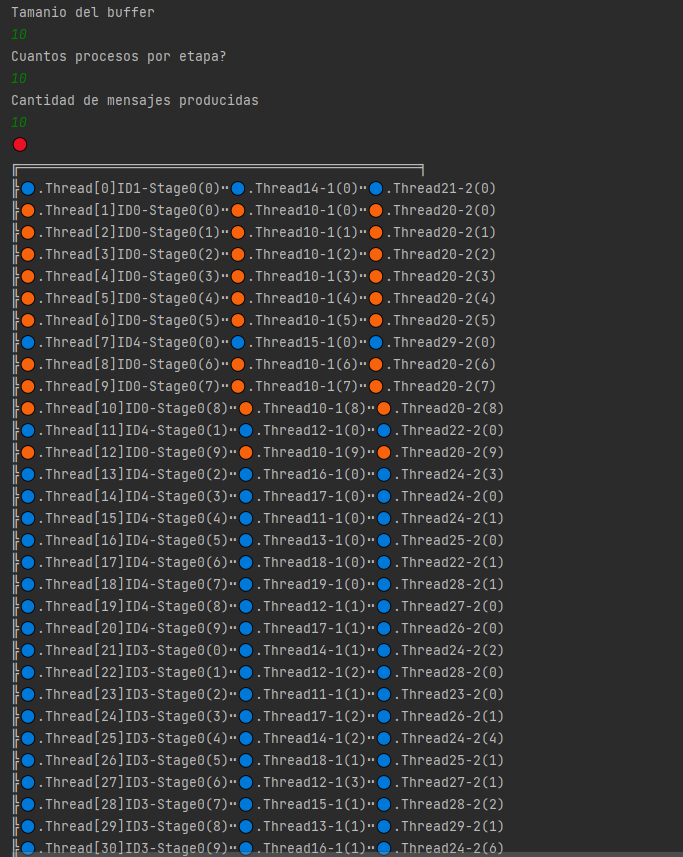
\includegraphics{10-10-10.PNG}

\subsubsection{3-3-3}
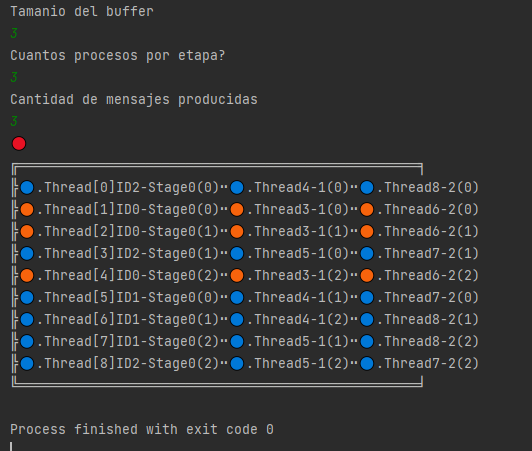
\includegraphics{3-3-3.PNG}

\subsubsection{5-5-5}
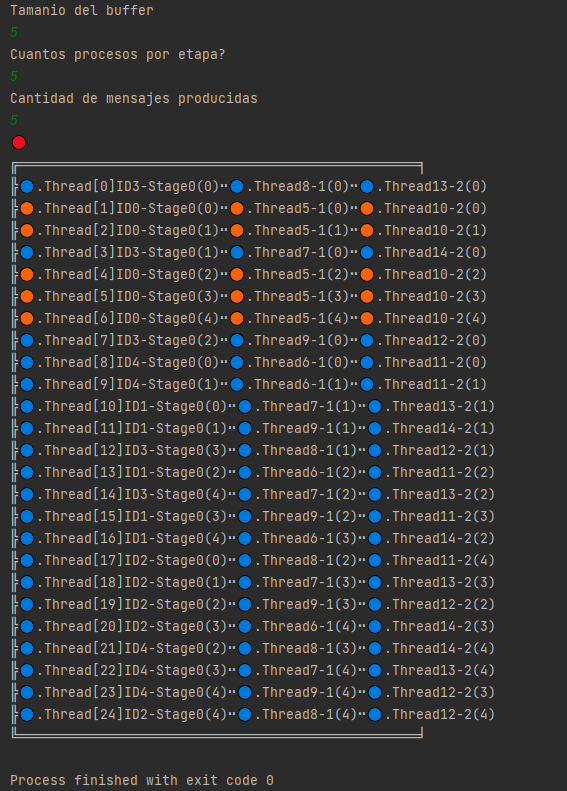
\includegraphics{5-5-5.PNG}

\section{Glosario}
\paragraph{Función Lambda}

\paragraph{Objeto anónimo}


%------------------------------------------------
\end{document}
